\section{measurements}
\subsection{Calibration and preparation}
As it was already described we performed the calibration in order to maximize the amplitude of the
signal, which was the case for \\
\begin{align*}
     \mathrm{VCA} &= 1357 \qquad \text{(Amplitude of the RLC circuit)}\\
     \mathrm{VCO} &= 1417 \qquad\text{(Frequency of the RLC circuit)}\\ 
     \mathrm{Offset} &= 1500 \qquad\text{(Offset for shifting the signal)}\\
\end{align*}
For the given constraints of the experimental setup see figure~\ref{fig:setup1}.
\begin{figure}[htpb]
    \centering
    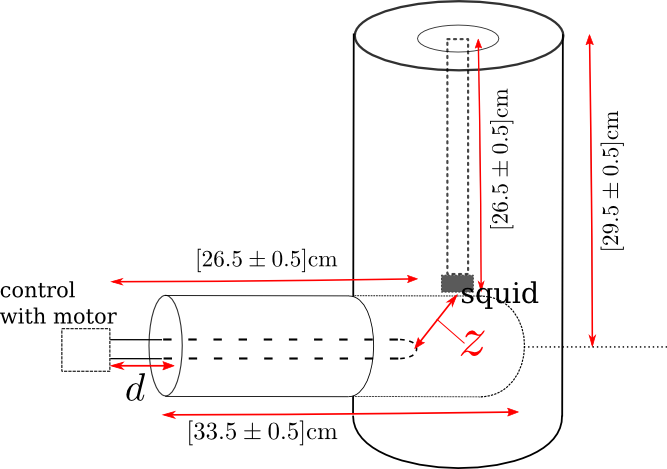
\includegraphics[width=0.8\linewidth]{figures/setup1}
    \caption{Experimental constraints, which we measured before the experimental procedure. The squid
    is connected to the controlling unit, whose output we observe on the oscilloscope. The oscillscope
    is additionally connected to the computer in order for us to analyze the output of the squid even further.}
    \label{fig:setup1}
\end{figure}
\\\\
We have measured the radius of the coil to be 
\begin{equation}
r = \frac{d}{2} = (2.0 \pm 0.25) \mathrm{mm}
\end{equation}

